\appendix{A Motivating Scenario}
\label{scenario}

While the \emph{LDS SCI} is helpful for the aspiring erudite of LDS content, there is currently no recommendation system for the discourses: when a user finds an interesting discourse, there is no quick, simple way to find similar/related discourse. Although the LDS website has some modern GC discourses tagged with topics, such topics are currently provided on a per-year basis only, so the discourses tagged with each topic tend to be sparse. This works when members of the LDS church want to focus on the most recent discourses only. Even with URL manipulation, attempts to expose topics for all GC discourses rather than by year do not work (\url{https://www.lds.org/general-conference/topics/2015/10} vs. \url{https://www.lds.org/general-conference/topics/})--and result in the topic index for the most recent session of GC. Sparseness for the discourses in a given topic are apparent in Figure \ref{fig:oct_2015_topics}--most topics only have 1 associated discourse and therefore have no number next to the topic’s title.

\begin{figure}[hhhhhtb]
	\centering
		%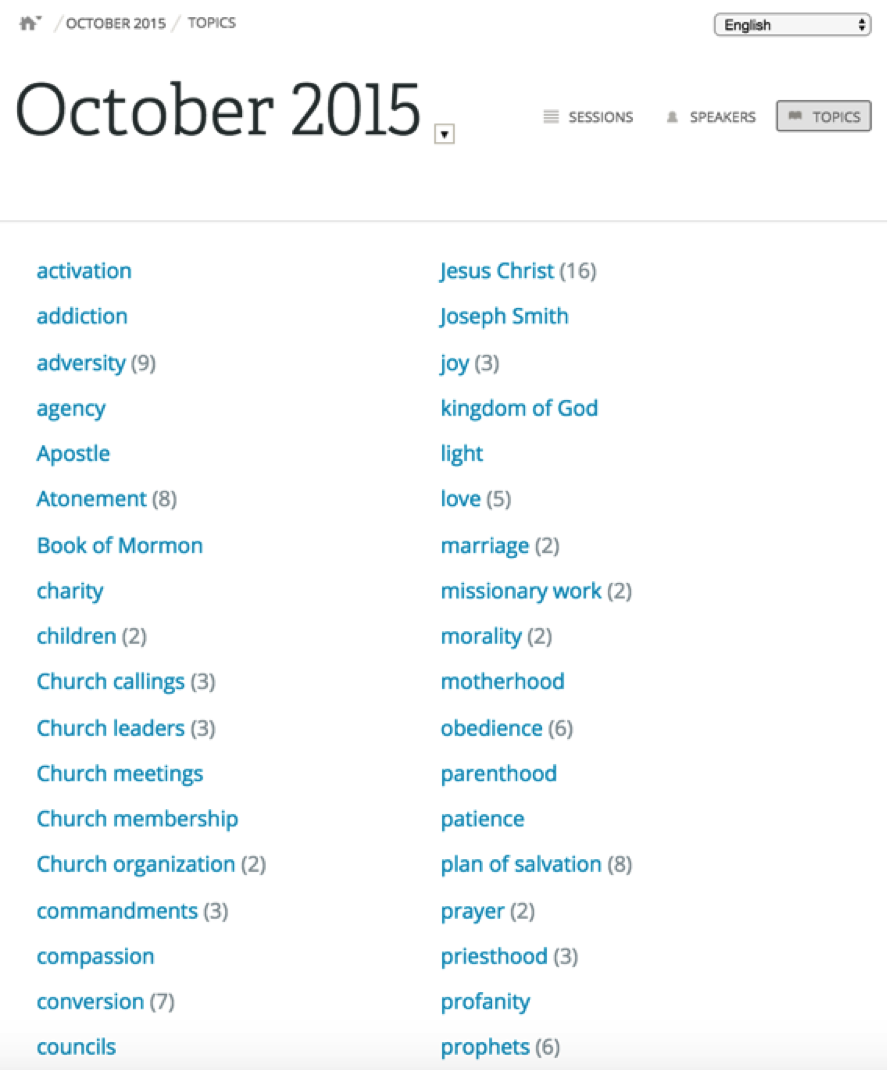
\includegraphics[width=4.5in,natwidth=410,natheight=542]{figures/oct_2015_topics.png}
		\caption[\url{LDS.org} 2015 Topics]{
			\url{LDS.org} 2015 Topics
		}
	\label{fig:oct_2015_topics}
\end{figure}

Therefore, for users of \url{LDS.org}, when a reader enjoys a particular discourse, it is difficult to locate all discourses on a given topic. It is theoretically possible to peruse every session of GC (as far back as 1971) looking for the topic in every year. The task requires a lot of clicking and will not work for discourses published before 1971 since they are not exposed online at \url{LDS.org}.

Beyond the per-year topic index provided by \url{LDS.org}, \url{LDS.org} does have a Gospel Topics index at \url{https://www.lds.org/topics/}. Under some topics, there are discourses that are selected for the topic, but they don’t promise to be results of a recommendation system that is routinely updated--and expanding the lists to see more is not possible.

\emph{LDS SCI} has discourses by topic, but was manually created and only accounts for discourses in the Journal of Discourses, which were published in the 1800’s. For those interested, digital images of the Journal of Discourses are available from the BYU online collections at \url{http://contentdm.lib.byu.edu/cdm/search/collection/JournalOfDiscourses3}.

To review, \url{LDS.org} has 2 topic indexes, one of which focuses on a per-year approach for post-1971 GC talks, the other of which appears to have been manually created. \emph{LDS SCI} has a topic index, but only for very early discourses. For a superficial study of a topic, this might be sufficient, but when one wants to reach farther than the most recent or least LDS materials--namely those in the middle--there is no search engine--and none which promises to be automatic, automatically updated, and interactive.

In the past 2 years, the query engine provided by both \url{LDS.org} and \emph{LDS SCI} have been enhanced significantly, but they still leave something to be desired: simplicity and ease of use. Dr. Liddle who built \emph{LDS SCI} has said that \emph{LDS SCI} uses a Lucene query engine, which employs a \emph{TF-IDF} search algorithm. The \url{LDS.org} engine seems to work similarly, except that it can detect phrases such as ``in talks'' and use those to automatically select to search only through discourses rather than through all LDS written materials exposed online. %[...more on how LDS SCI search engine works...]

Take for example the search query ``word of wisdom'' (without quotes in the search). This is a phrase which is more recent history of the LDS church has come to refer to a law of health. The search results look promising (shown in Figure \ref{fig:sci_results}).

\begin{figure}[hhhhhtb]
	\centering
		%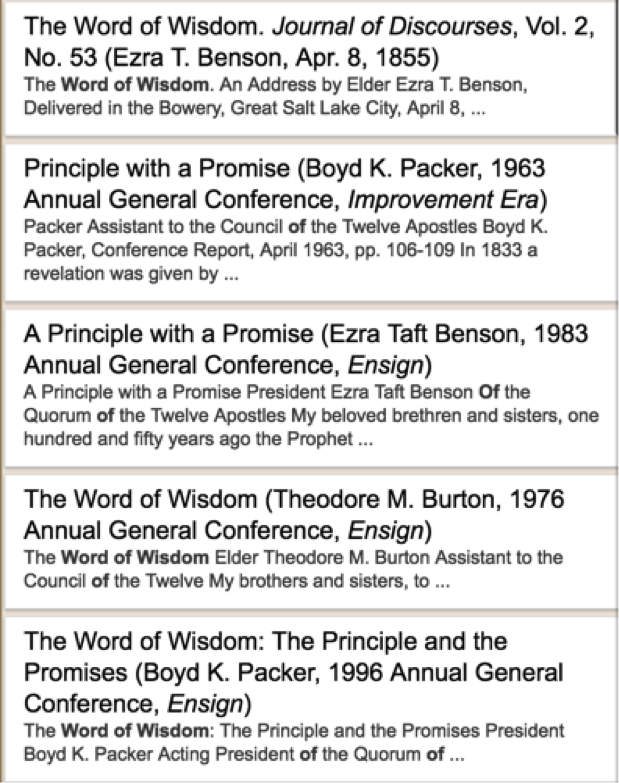
\includegraphics[width=3.5in,natwidth=310,natheight=442]{figures/sci_results.png}
		\caption[Top SCI Query Results for the search \textit{Word of Wisdom}]{

		}
	\label{fig:sci_results}
\end{figure}

But one would expect to see something by Joseph Smith Jr. to rank at the top. The confounding factor here is that ``word of wisdom'' is a modern naming convention. % TODO: Fact check this!
The word of wisdom was ``[r]evelation given through Joseph Smith the Prophet, at Kirtland, Ohio, February 27, 1833.'' (D\&C 89 Header). The earliest usage of the phrase ``word of wisdom'' in print we could find is 1873--40 years after it was revealed \citep{missing}. %TODO: \cite The Word of Wisdom—Education by President George A. Smith.

Unfortunately, without a way to determine what topics exist within all the GC discourses, there is no way for a query system to expand queries like this one. Unfortunately, even if the user does happen to find a discourse that is a pleasing match to the query, there is currently no recommendation system from that point to suggest other related discourses--just existing links and the other results for the query.

If the user were to filter to only scriptures, they would find more than 20k matches as shown in Figure \ref{fig:sci_results_20k}.

\begin{figure}[hhhhhtb]
	\centering
		%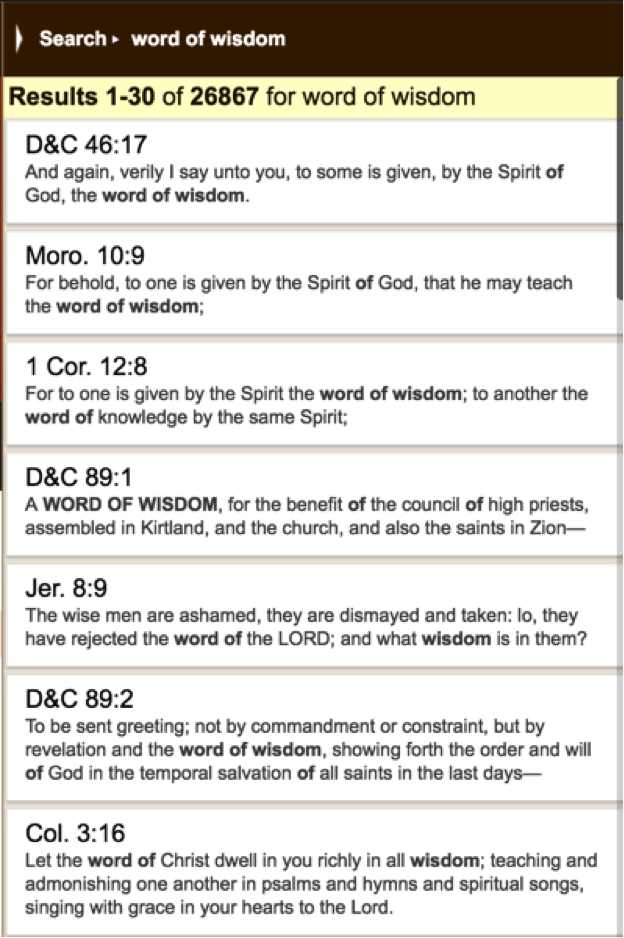
\includegraphics[width=3.5in,natwidth=310,natheight=442]{figures/sci_results_20k.png}
		\caption[20k+ SCI Results]{

		}
	\label{fig:sci_results_20k}
\end{figure}

Of those, the first one that refers to directly to a law of health is the 4th result. \url{LDS.org}, when performing the same search ranks the result referring to the law of health as the 4th result (\url{https://www.lds.org/scriptures/search?type=verse&query=word+of+wisdom}), but does so with only 39 total results. These are results that I was able to find because I understood how the search engine works. When one doesn’t know when to put quotes or doesn’t know what they are looking for, the task is more difficult, depending on the engine used. For example, when the entire query is run with quotes around it in \emph{LDS SCI}, the number of results drops from the 20k down to 7 in \emph{LDS SCI}; in \url{LDS.org}, from 39 to 8 (\url{https://www.lds.org/scriptures/search?type=verse&query="word+of+wisdom"}). Search relevance is an entire area of research and it is no wonder that companies that are able to do well in this area are able to profit from it (e.g. Microsoft with \url{https://bing.com} and Google with \url{https://google.com}). Query systems are a natural way to 'ask' a computer questions and receive results, but are obviously lacking in features.

While search query optimization would be one way to improve this area, I chose to augment the \emph{LDS SCI} toolset with recommendation features. The idea was that once a reader locates a discourse of interest, a user should be able to quickly locate similar discourses by viewing a pre-computed list of related/similar documents as a list. The list could default to displaying 5 results, but the user could interact with the list and request additional results. %There are many ways to approach this that I will explain.